\begin{frame}{Simulation Numérique et Maillage : Définition}
  
    \textbf{Simulation Numérique:}
    \begin{itemize}
      \item Technique utilisant des ordinateurs pour reproduire le comportement d'un système via des modèles mathématiques.
      \item Émergence : 1940s (projet Manhattan).
    \end{itemize}
    
    \pause
    \vspace*{.3cm}
    \textbf{Maillage:}
    \begin{itemize}
      \item Division d'un domaine en éléments discrets pour l'analyse numérique.
      \item Émergence : 1950s (Boeing, Nasa, ...).
    \end{itemize}
  
\end{frame}


\begin{frame}{Simulation Numérique et Maillage : Exemple}
    \textbf{Propagation d'onde mécanique dans un téléphone}
    %\end{block}
    
    \begin{columns}
        \begin{column}{0.4\textwidth}
            \begin{itemize}
                \item Le maillage facilite la modélisation du stress mécanique.
                \item La qualité du maillage impacte la simulation 
            \end{itemize}
            \begin{center}
                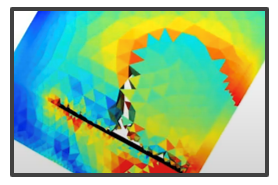
\includegraphics[width=.9\linewidth]{img/new_images/convergence_depend_simu.PNG}
            \end{center}
        \end{column}
        \begin{column}{0.6\textwidth}
            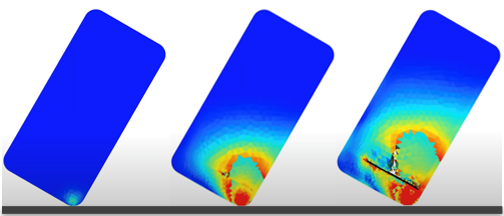
\includegraphics[width=\linewidth]{img/new_images/phone_drop.png}
            Chute d'un téléphone [ANSYS]\\
            \scriptsize{\url{https://www.youtube.com/watch?v=gVz3eJrMMmM}}
        \end{column}
    \end{columns}
\end{frame}

\begin{frame}{Pourquoi des maillages hexaédriques ?}
    \begin{columns}[T] % align columns
        \begin{column}{.4\textwidth}
            \textbf{Pour les simulations de grandes déformations hyper-élastiques :}

            %Pour la mécanique de matériaux hyper-élastiques:
            \begin{itemize}
                \item En 2D, maillage quadrilatère plutôt que triangulaire
                \item En 3D, maillage hexaédrique plutôt que tétraédrique
            \end{itemize}
        \end{column}%
        
        \begin{column}{.6\textwidth}
            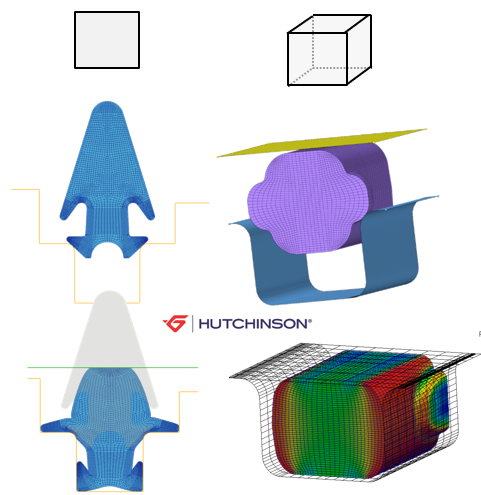
\includegraphics[width=1.\linewidth]{img/new_images/simu_hutchinson_2d3d.png}
        \end{column}
    \end{columns}
\end{frame}

\begin{frame}{Maillages Quadrilatères et Hexaédriques : Challenges}
    \begin{columns}[T] % align columns
        \begin{column}{.5\textwidth}
            %Un maillage non-structuré pose des problèmes de convergence. \vspace*{.2cm}\\
            \textbf{Qualité du maillage}
            \begin{itemize}
                \item Alignement avec les bords
                \item Angles proche de 90°
                \item Peu de singularités
            \end{itemize}
            
            \textbf{Pas d’algorithme générique}
            \begin{itemize}
                \item Intervention humaine
                \item Subdivision manuelle en blocs structurés
                \item Plusieurs semaines/mois pour construire un maillage
            \end{itemize}
        \end{column}%
        
        \begin{column}{.5\textwidth}
            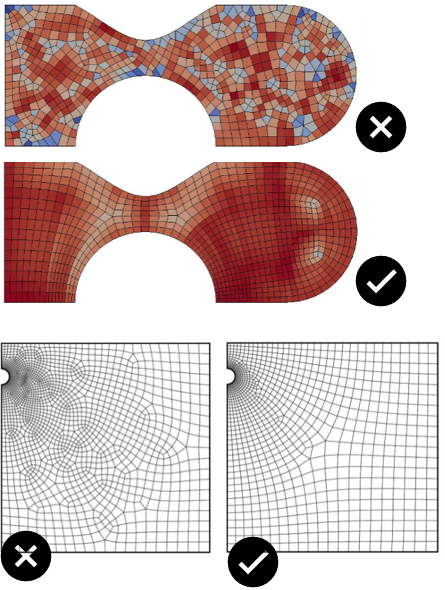
\includegraphics[width=\linewidth]{img/new_images/qualite_maillage_important.PNG}
        \end{column}
    \end{columns}
\end{frame}

\begin{frame}{Objectif de la thèse}
    \centering
    \textbf{Automatiser la génération de maillage quad/hex de haute qualité pour les simulations de grandes déformations}.\\ \vspace{1em}
    \only<1>{ 
        \begin{tabular}{c|c}
            \textit{Entrée} : Maillage tri & \textit{Sortie} : Maillage quad $< 1$ min\\ \hline \\
             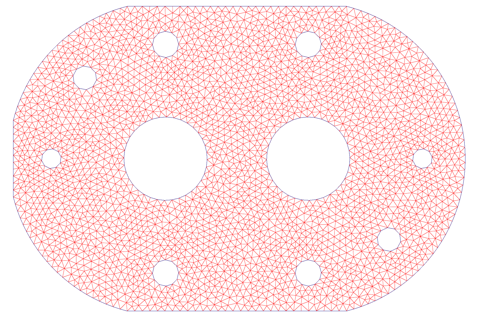
\includegraphics[width=0.45\linewidth]{img/new_images/entree_maillage_tri.png} &  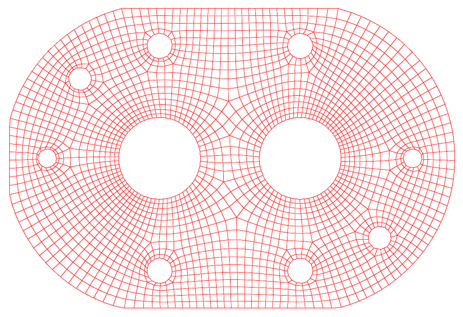
\includegraphics[width=0.45\linewidth]{img/new_images/sortie_maillage_quad.png} \\
        \end{tabular}

    }
    \only<2>{
        \begin{tabular}{c|c}
            \textit{Entrée} : Maillage tétra & \textit{Sortie} : Maillage hex $< 1$ min\\ \hline \\
             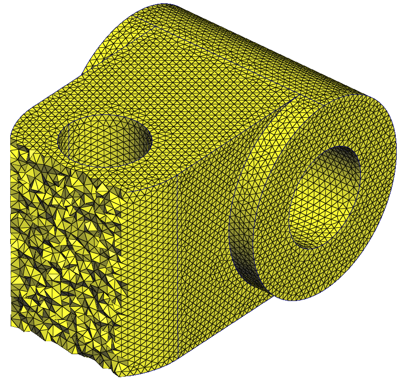
\includegraphics[width=0.45\linewidth]{img/new_images/entree_maillage_tet.png} &  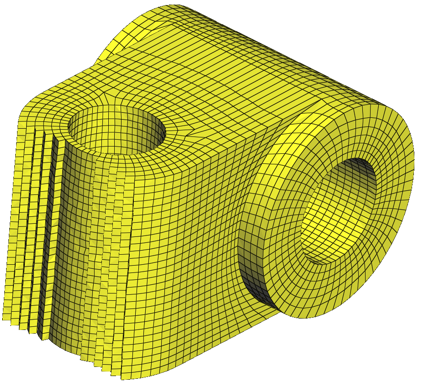
\includegraphics[width=0.45\linewidth]{img/new_images/sortie_maillage_hex.png} \\
        \end{tabular}
    }
\end{frame}

\begin{frame}{Approche générale de la méthode en 2D}
    \centering
    \textbf{Paramétrisation globale}
    
    %\vspace{1em}
    
    \begin{figure}
        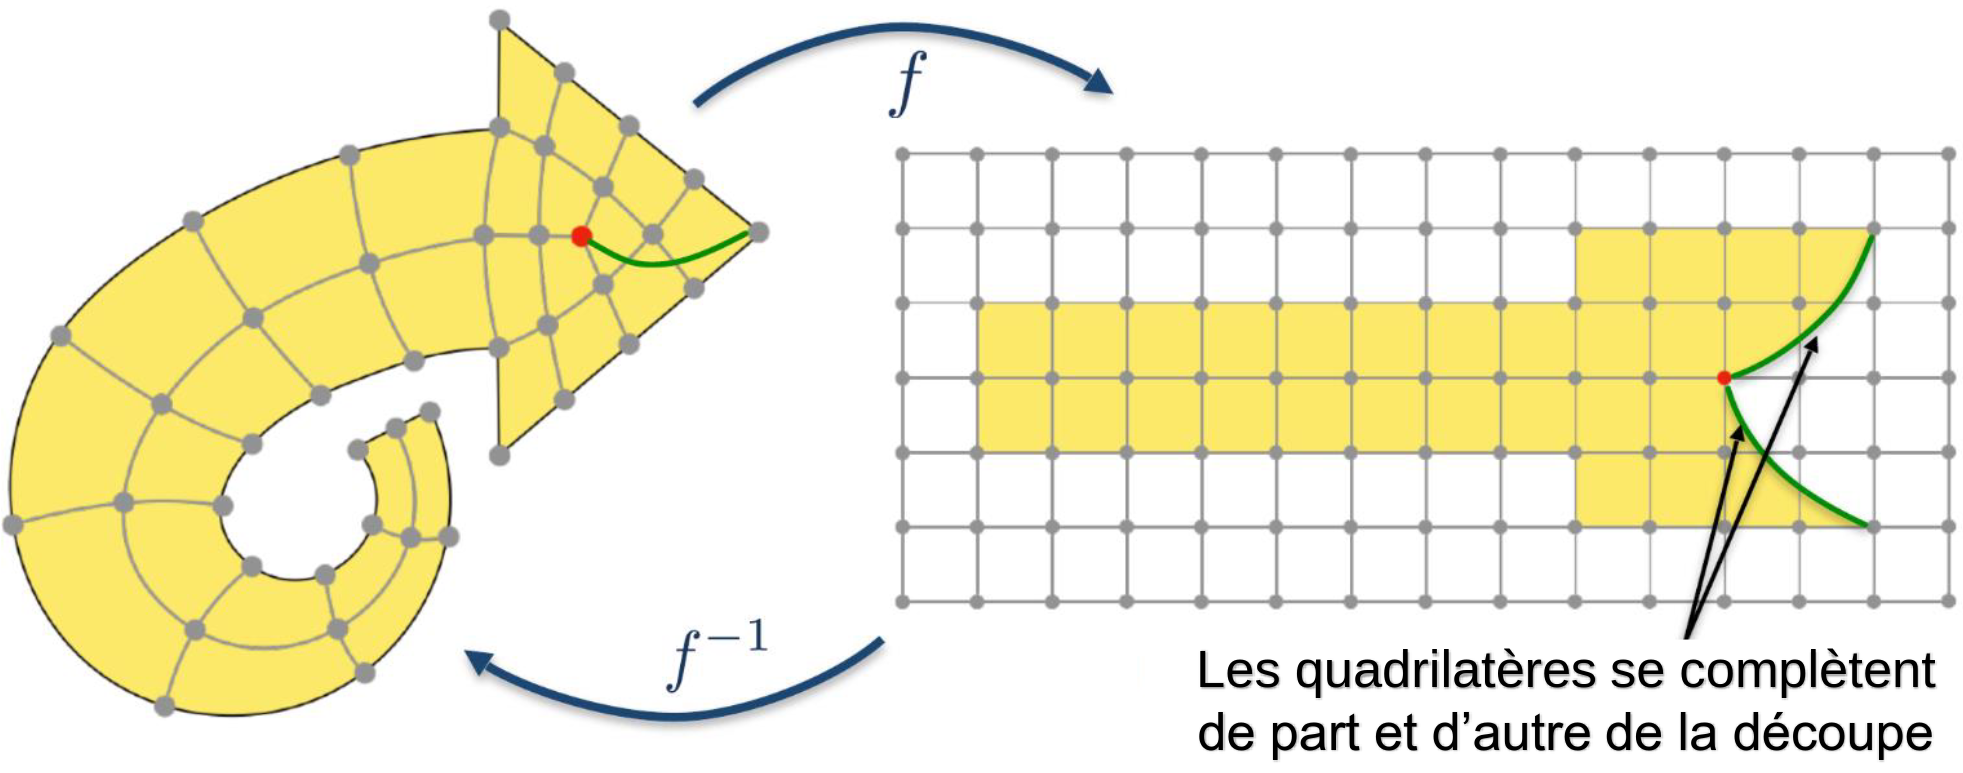
\includegraphics[width=1.\linewidth]{img/new_images/gp_arrow_ex.png}
    \end{figure}

    \begin{itemize}
        \item Paramétrisation $f$ d'un domaine 2D vers une grille régulière.
        \item $f^{-1}$ permet de déposer la grille sur le domaine initial.
    \end{itemize}
\end{frame}

\begin{frame}{Méthode Quadcover pour calculer un maillage quadrilatère}
    \begin{columns}[c] % align columns
        
        \begin{column}{.7\textwidth}
            \textbf{Méthode utilisant un champ de repère}
            \vspace{1em}
            \begin{enumerate}
                \item Calcul champ de repère
                \begin{itemize}
                    \item Oriente les quadrilatères
                    \item Positionne les singularités
                \end{itemize}
                \vspace{.5em}
                \item Algorithme Quadcover
                \begin{itemize}
                    \item Calcule une paramétrisation globale
                    \item Extrait un maillage quadrilatère
                \end{itemize}
            \end{enumerate}
        \end{column}%
        
        \begin{column}{.3\textwidth}
            \begin{figure}
                \centering
                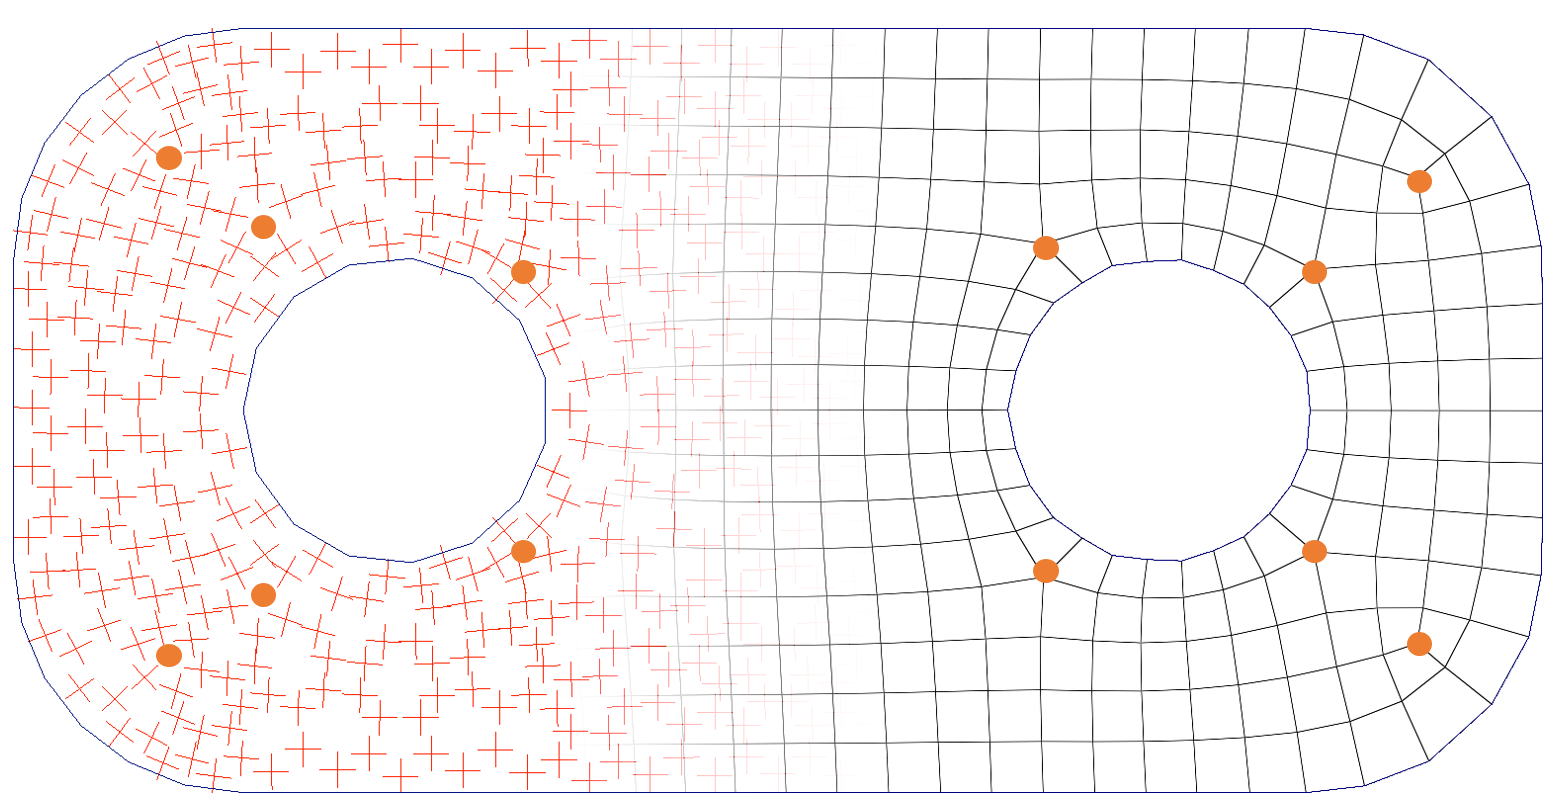
\includegraphics[width=1.8\linewidth, angle=-90]{img/quadsimu/singus.PNG}
            \end{figure}
        \end{column}
        
    \end{columns}
\end{frame}

\begin{frame}{Extraction de deux champs de vecteurs \blue{$\vec{a}$} et \red{$\vec{b}$}}
    \centering
    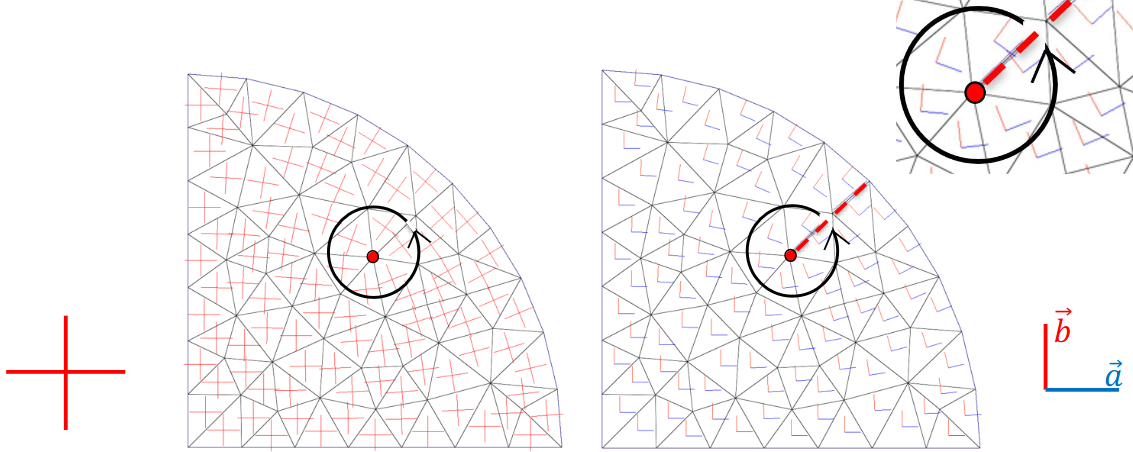
\includegraphics[width=\linewidth]{img/new_images/ff_to_vf.png}
\end{frame}

\begin{frame}{Algorithme Quadcover}
    \begin{columns}
        \begin{column}{0.5\textwidth}
            \textbf{Intégration de \blue{$\vec{a}$} et \red{$\vec{b}$} en champs scalaires \blue{u} et \red{v} }
            \begin{itemize}
                \item Calcul de \blue{u} qui minimise \[\int{ |\nabla{\blue{u}} - \blue{\vec{a}}|^2 }\]
                \item Calcul de \red{v} qui minimise \[\int{ |\nabla{\red{v}} - \red{\vec{b}}|^2 }\]
                \item De part et d'autre de la découpe (\blue{u}, \red{v}) est rotationné de 90°
            \end{itemize}
        \end{column}
        
        \begin{column}{0.5\textwidth}
            \centering
            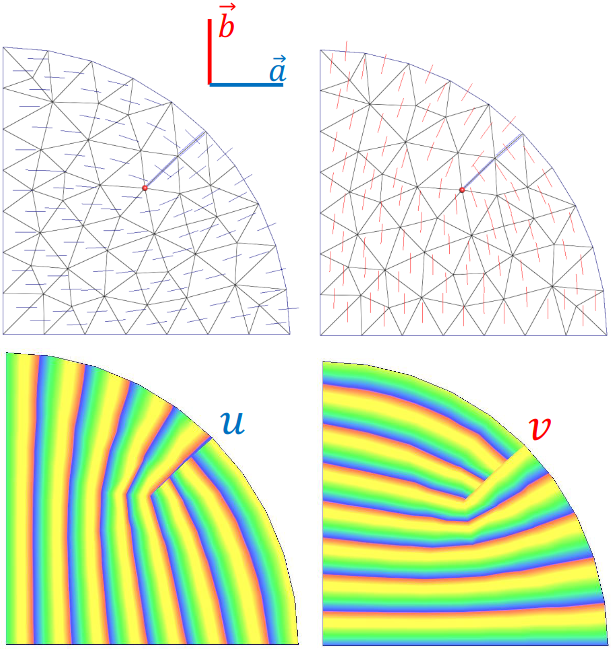
\includegraphics[width=\linewidth]{img/new_images/vf_to_sf.png}
        \end{column}
    \end{columns}
\end{frame}



\begin{frame}{Algorithme Quadcover}
    \centering
    \begin{itemize}
        \item On obtient une paramétrisation du domaine \[f(x,y) = (\blue{u(x,y)}, \red{v(x,y)})\]
    \end{itemize}
    
    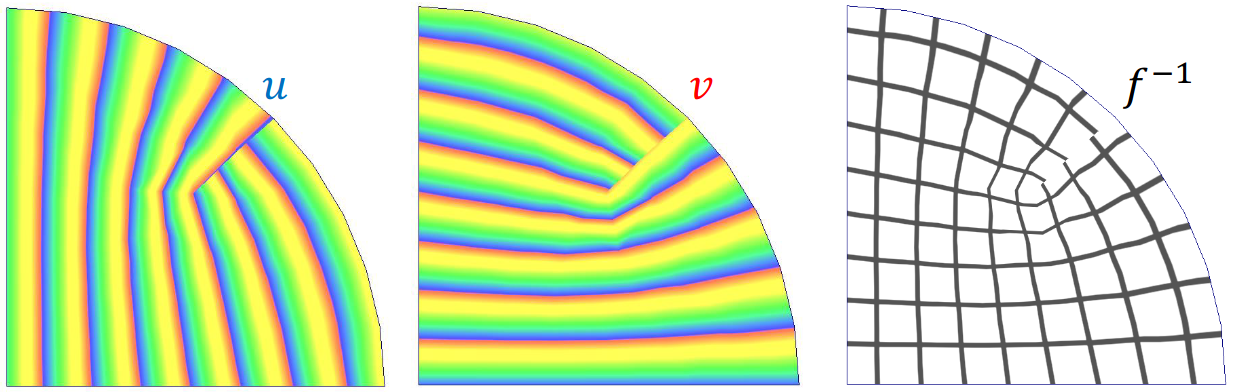
\includegraphics[width=\linewidth]{img/new_images/u_v_forme_f.png}
    \vspace{-1em}
    \begin{itemize}
        \item Problème : Les lignes de la grille par $f^{-1}$ se situent sur les lignes entières de $\blue{u}$ et $\red{v}$
        qui ne sont pas alignés avec le bord.
    \end{itemize}
\end{frame}

\begin{frame}{Quantification de \blue{u} et \red{v} sur des valeurs entières}
    \begin{itemize}
        \item Chaque bord devient une valeur entière pour $\blue{u}$ ou $\red{v}$
        \item Chaque découpe devient une translation entière pour $\blue{u}$ et $\red{v}$
        \item Chaque singularité est une valeur entière pour $\blue{u}$ et pour $\red{v}$
    \end{itemize}
    
    \vspace{1em} % Espacement, à ajuster selon vos besoins
    \centering
    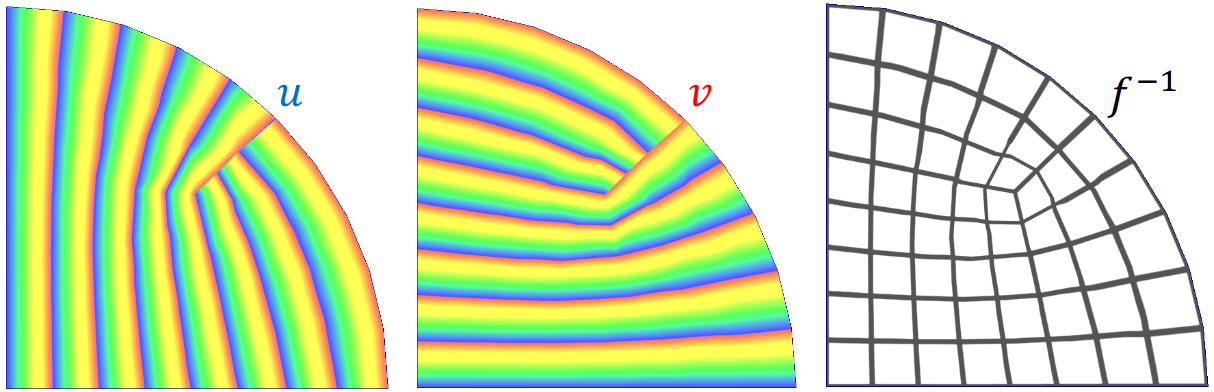
\includegraphics[width=\linewidth]{img/new_images/uv_quantizee.png}
\end{frame}